
\subsection{PARTICLE IMAGE VELOCIMETRY}

$PIV$ is a technique to determine the  velocity field of objects from a stream of images\cite{Bastiaans}.
The result of the $PIV$ is given as a vector field, showing for each particle the direction, sense and intensity of velocity. 
Moreover, the $PIV$ can be calculated for different objects in the same image.
For this purpose, the $PIV$ technique divides the frame 1 in regions (particles), after frame 1 and 2 are correlated 
using comparative method, so a vector or a field of vector is generated that represent the displacement. Thus, we have 
displacement and time of computing, applying of conception of derivate it is possible to estimate relative velocity.

\begin{figure}[H]
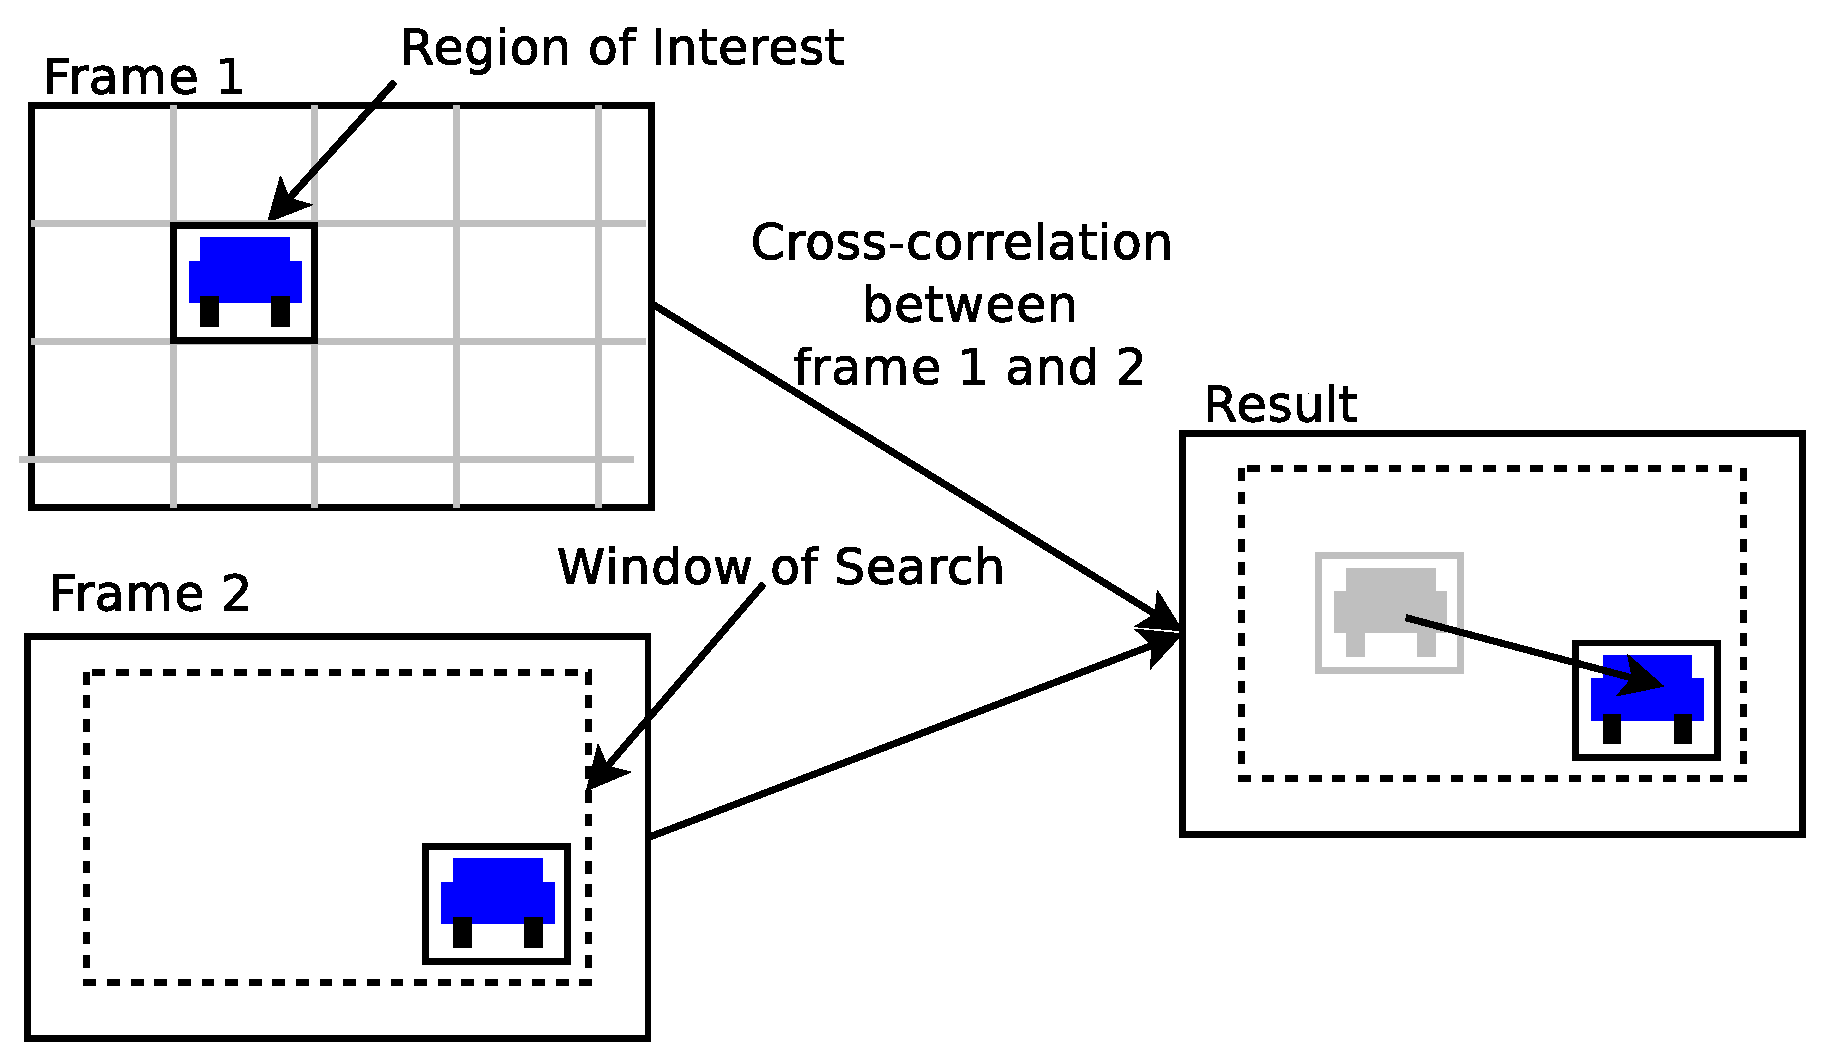
\includegraphics[width=\columnwidth]{images/explanationPIV.eps}
\caption{The PIV operation comparing two frames}
\label{fig:twoframes}
\end{figure}

The Fig. \ref{fig:twoframes} shows how PIV works and also demonstrates the relation between Region of Interest (ROI) and 
Window of Search (WOS). WOS involves ROI because WOS is considered the possibles regions that object could be. 
WOS don't need necessary fill whole image. If WOS is large, so we have an augment of computing but 
if WOS is small, object can be lost. In our application, we determine WOS from 1,5 of ROI. For example, 
if ROI is 200x300 so we have WOS of 300x450. It means object will be in anywhere in this WOS. This consideration can be
proven by testes in environment of low velocity of objects (velocity in cities and roads).

\begin{figure}[H]
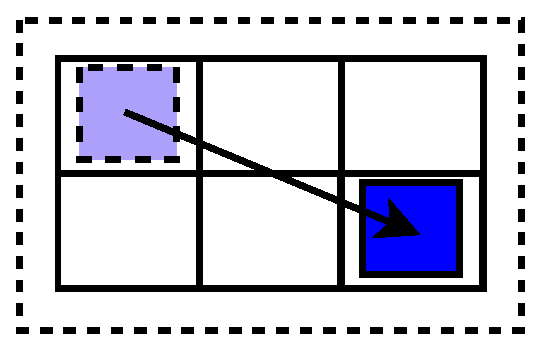
\includegraphics[width=\columnwidth]{images/WOSdivided.eps}
\caption{WOS is divided in windows of same dimensions of ROI}
\label{fig:WOSdivided}
\end{figure}

ROI is one of most important part of PIV, because it contains target. An window of same dimension of ROI is displaced
along of whole WOS in frame 2, like showed in Fig. \ref{fig:WOSdivided}. One comparison is done and assigned a value in each displacement. 
When process finishes, the more height value is considered the new place of ROI. It means that object displaced of initial 
position in frame 1 to found position in frame 2.